\documentclass[12pt]{article}
\usepackage{fullpage, graphicx, psfrag}
\usepackage{epsfig}
\usepackage{epstopdf}
\usepackage{color, soul}
\usepackage{graphics}
\usepackage{pgf,pgfarrows,pgfnodes,pgfautomata,pgfheaps}
\usepackage{graphicx}
\usepackage{setspace}
\usepackage{amsmath,amsfonts,amssymb,amsthm}
\usepackage{fancyhdr}
\usepackage{multirow}
\usepackage{pdfpages}
\usepackage[colorlinks]{hyperref}
\usepackage{longtable}
\usepackage{listings}
\usepackage[margin=0.5in]{geometry}
\usepackage{epsfig}
\usepackage{epstopdf}
\usepackage{color}
\usepackage{graphicx}
\usepackage{pdfpages}

\hypersetup{linkcolor=blue}


\thispagestyle{empty}
%\pagestyle{myheadings} \markright{}
\renewcommand{\baselinestretch}{1.75}
\setlength{\topmargin}{0in} \setlength{\textheight}{8.75in}
\setlength{\textwidth}{6.3in}
 \setlength{\oddsidemargin}{0in}
\partopsep=-0.10in

\addtolength{\oddsidemargin}{-0.875in}
\addtolength{\evensidemargin}{-0.875in}
\addtolength{\textwidth}{1.5in}
\lstset{framesep=10pt}
\lstset{xleftmargin=10pt, xrightmargin=10pt}
\lstset{breaklines}

\newcommand{\mathb}[1]{\mbox{\boldmath$#1$}}
\newcommand{\bx}{\mbox{\boldmath$x$}}
\newcommand{\bX}{\mbox{\boldmath$X$}}
\newcommand{\by}{\mbox{\boldmath$y$}}
\newcommand{\bb}{\mbox{\boldmath$b$}}
\newcommand{\bY}{\mbox{\boldmath$Y$}}
\newcommand{\bv}{\mbox{\boldmath$v$}}
\newcommand{\bz}{\mbox{\boldmath$z$}}
\newcommand{\bw}{\mbox{\boldmath$w$}}
\newcommand{\bW}{\mbox{\boldmath$W$}}
\newcommand{\bbeta}{\mbox{\boldmath$\beta$}}
\newcommand{\bgamma}{\mbox{\boldmath$\gamma$}}
\newcommand{\blambda}{\mbox{\boldmath$\lambda$}}
\newcommand{\btheta}{\mbox{\boldmath$\theta$}}
\newcommand{\bphi}{\mbox{\boldmath$\phi$}}
\newcommand{\sumk}{\sum_{i=1}^k}
\newcommand{\maxk}{\max_{1\leq i \leq k}}
\newcommand{\mink}{\min_{1\leq i \leq k}}
\newtheorem{theorem}{Theorem}
\newtheorem{lemma}{Lemma}
\newtheorem{corollary}{Corollary}

\numberwithin{figure}{section}

\begin{document} \begin{center}{\large{\sf Summary of Obesity and Basic Vital Sign Data from NHANES}}\end{center}
\sloppy
\begin{spacing}{1.70}

\begin{center}
{\bf {\sf Authors:}}\\
{\sf CSC 595 \\
...}\\
\end{center}

\end{spacing}

\setcounter{page}{1}

\pagenumbering{arabic}
\setcounter{section}{0}

\newpage
{\section{Introduction and Data Description}}
{\subsection{Data Introduction and Overall Summary}}

The NHANES is a large scale longitudinal database created by the Centers for Disease Control and Prevention (CDC) to collected data from a sub-sampling of the United States population.  The data includes interview data, physical examinations to include vital signs (systolic and diastolic blood pressure, height, weight, BMI, ...) as dental information, laboratory measurements (i.e. glucose or HBA1C values for diabetes), and demographics information.  The purpose of this data is set national standards (i.e. BMI percentile measurements standardized by age and sex), track health data for diseases like cardiovascular disease or diabetes to shape public policy, or provide data for international research organizations and academic institutions for many purposes.  Please see the following example of areas which have used this data: Iranpour at al (2019) looked at the inverse relationship between amount of caffeine consumed and symptoms of depression; Wang at al (2018) looked at the relationship between the cadmium in the blood and both blood pressure and obesity; Howell et al (2017) looked at the mortality rate of Mexican American adults in relation to their BMI/BMI percentile as well as demographic information.

The focus of the interactive tool as well as this report is to provide summaries of obesity data collected in NHANES.  Obesity is a serious problem as documented by the CDC and World Health Organization (WHO) which has led to an increase in many diseases ranging from cardiovascular disease to diabetes worldwide.  Hales, Carrol, Fryar, and Ogden (2017) documented the incidence of obesity in the united states based on different demographic data based on a publication within that organization from 20165- 2016.  This paper presented this information through bar charts to overall counts by demographic groups as well as line charts to show the incidence rates within the time frame of 2015-2016. They also showed line plots overtime from 1999 to put these results in a general context.  Thompson et al (2007) explored the impact of childhood obesity upon later health effects and identified risk factors for long term health.  In this study the long terms impacts for how the development of cardiovascular disease were examined to see impact upon children as well as effects within adulthood.  The Centers for Disease Control and Prevention looked at incidence of diabetes with regards to many risk factors including obesity (2011).  Ford ES (2005) summarized the risk factors for both cardiovascular disease and diabetes and indicated the link between both diseases and obesity.

This interactive tool will provide a summary of the prevalence of obesity using the NHANES data.  This will due this for different demographics variables to show the prevalence based on variables like age.  Variables were also generated showing the continuous variables like age, height, and weight were binned for use in tree or treemap plots.  It was felt that from the clinical perspective these were good as they mimicked clinical flow diagrams.  Thus this would be good visualization approaches based on how clinicians look at diagnosis strategies based on flow charts.  The purpose of the data was the emphasize summary of obesity in a way meant to reflect clinical judgement.  Once they clicked on an element of the space filling plot they could see the sub-statistics for the additional selectable variables through bar charts to gain a better understanding of the relationship between the two.


\vspace{5 mm}

{\subsection {Data Description}}

The data included in our combined dataset includes the following:
\begin{longtable}{|p{5cm}|p{1.4cm}|c|p{2cm}|p{6.5cm}|}
\hline
\multicolumn{5}{|c|}{Summary of Variables}\\
\hline
Variable Name&Units&Type&Labels&Description\\
\hline
Sequence Number &&Categorical& & Primary key for all csv files for NHANES\\
\hline
Age &Years&Integer& & Age at time of the vital sign measurement in years\\
\hline
Age Grouping&&Categorical&21-30, 31-40,... &Derived based on ten year intervals\\
\hline
Height&cm&Float with 1-decimal& & \\
\hline
Height Grouping&&Categorical&151-175, 176-200, ...& Derived\\
\hline
Weight&kg&Float with 1-decimal&  & \\
\hline
Weight Grouping&&Categorical&71-80, 81-90, ...& Derived\\
\hline
BMI&$\frac{kg}{m^2}$&Float with 1-decimal&  &Derived based on height and weight \\
\hline
Systolic BP&$mmHg$&Float with 1-decimal&  & \\
\hline
Diastolic BP&$mmHg$&Float with 1-decimal&  & \\
\hline
Total Cholesterol&$\frac{mg}{dL}$&Integer&  & \\
\hline
Obesity&&Boolean& TRUE, FALSE &TRUE = Obese, FALSE = Not Obese \\
\hline
\end{longtable}

The data contains the overall key as well as important vital sign variables such as height, weight, BMI, and blood pressure.  Some variables have been derived to create categorical groupings.  This makes sense as there may be much change year to year for most people under 40 (in the elderly population there would be more impact upon health even from year to year or even month to month).  Yet there are significant medical issue which appear from decade to decade as the health problems for a 20 year old and different than a 40 year old.  They also allow for these variables to be used in our visualizations such as treemaps.  The same is true for the height and weight groupings.  The categorical bins allow for the binning of subjects in the space filling approaches to expand to more detailed data on obesity within those groupings.  The treemaps would show the counts based on space filling for variables like height, weight, or age by bins whereas the bar charts would show the relationship between to the factors based on percentages to obesity and cholesterol. 

A few things to note on the relationship between obesity and the variables.  There is a clear relationship between BMI, age, gender, and obesity.  Using the CDC website [9] obesity can be defined as a function of BMI with BMIs 30 or higher classified as obese and BMIs between 25.0 and 29.9 as overweight.  For teens and children BMI is not calculated in the same manner as the CDC indicates this is a function of age and gender.  It should be noted that the categorical representation by scientists of this variable as opposed to just relying upon the continuous values.  Obesity is based on the BMI percentile for children and a teen or child would be considered obese if their BMI percentile was above the $95^{th}$ percentile for their age and gender.  This is a standard value based on a teen or child's age or gender.  It is also clear that height and weight impact obesity as BMI is weight divided by height squared.  There should be a correlation between blood pressure and obesity but not as strong as the other variables.  There should be a positive correlation between hypertension (high blood pressure) and obesity.  Similarly there should be a positive correlation between total cholesterol (especially triglycerides) and obesity.  High and extreme levels of cholesterol (dyslipidemia, hyperlidemia, or hypertriglyceridemia) should have an increased risk for obesity.  Nonetheless both cholesterol and blood pressure should have a weaker relationship as there other factors impacting each such as stress and genetics.  Choi (2014) has an interesting paper looking at the relationship between obesity and different complication like diabetes and cholesterol issues based on a biological perspective.  This would explain biologically the correlations between the various issues.  All variables chosen would be highly correlated to somewhat correlated and show-up in the visualization as expected from the layman's perspective.

{\subsection {Data Cleaning}}
Even though the NHANES data is contained is various databases as .csv files (lab data, vital signs data, concomitant medication data, demographics data, ...) not much was required for data cleaning.  All databases had a common linkage based on the sequence number (primary key) which connected all the databases with demographics easily.  All that was needed was simple merging to get whatever demographics variables as needed.  For some continuous variables it was necessary to create a new categorical variables based on binning.  For example to make the different bins for cholesterol a new ordinal variable was created for each bin so they could be incorporated into the visualization easier.  No other data cleaning was done as the focus was on the visualization as opposed to outlier diagnostics or checking for data integrity.


\newpage


{\section{Description of Interactive Visualization Approach}}
The visualization was designed around the initial view being a treemap.  As described above this representation would be an approach familiar with clinicians who often use flow diagrams for diagnostics.  Also many clinical tables for variables like demographics would contain basic stats (counts, means, percentages) for all key variables.  This approach would mimic that table is a visual form.  The variables summarized would be things for subjects like race, age (numerical or categorical), height, weight, or history of specific illnesses as appropriate.  At the top of the form a radial button was added to select specific variables (age, height, or weight).  Once these are selected this will pick the overarching treemap structure by these groups from the dataset.  These treemaps would show the basic count data for each of these variables based on the categorical groupings.

The next approach was to expand each of these groups based upon the additional variables.  These included BMI, cholesterol, and obesity.  These would show the statistics based upon which rectangle of the treemap was selected and all displayed the percentages.  The splits were 0-17, 18-23, 24-29, 30-35, and 36-42 for BMI $\frac{kg}{m^2}$ , $<$160, 161-181, 181-200, 201-220, 221-240, and $>$240 for cholesterol in $\frac{mg}{dL}$, and "Obese" and "Not Obese" for obesity.  Originally pie charts were used to convey this information.  After the presentation these were changed to bar charts given that the interpretation of lengths is preferable to areas given we wanted to compare all groups within a given treepmap selection.


The treemap was fit in the center as this is the focus of everything.  It was important that this is the first thing seen as this is the most important and controlled element.  A title was placed on top describing which variable had been selected such as "Participants by Age".  It was hoped that this would avoid any confusion.  At the upper left but near the treemap is a box with radial buttons controlling which of the three variables are selected for the treemap among age, height, and weight.  This also had a colored border (purple-ish with a blue shadow) to contrast this with the white background making it easy to spot.  It was chosen to contrast with the white but not be too distracting using a distinct but mild coloring.  The bar charts (or original pie charts) would appear below based on the selection from the treemap.  Again this was to make it clear something would appear and it was felt people would see something appearing below as opposed to the right or left.  It was also felt these additional plots should be centered so that they fell just below the treemap.  Had they appeared in other spots this would have been awkward and having they align in a row makes reading easier.  Lastly at the bottom there is an endnote telling the user that all percentages have been rounded to the nearest unit.  This is important for two reasons: first it reminds the user that all numbers shown are estimated based on the data and not actual values and second it makes the table easier to read based on avoiding long numbers or the unscientific use of too many decimal places.  Using a key like this really tells the user not only the values but want rules were implemented for the calculations.

Now we will look at a few example and show some of the results for this work by comparing two groups: 21-30 and 51-60.  The first plot below shows the 21-30 and the second shows the 51-60.  Here we can see a difference in the number of people with obesity differs and the other elements shift as well.  Notice that the BMI bar charts shift to the left in the more people are in lower BMI bins for the 21-30 group.  Also note that the cholesterol numbers improve as well noting that correlation.  Again the bars shift to the right and more people are falling within the lower cholesterol bins for the 21-30 group.  This appears to be a common trend with age as subjects in the 18-20 and 21-30 tend to have better counts for all three bar plots than people in the higher age bins.  It is also worth noting the counts tend to level off after 30 with highest counts within the 51-60 group.  It is worth noting the numbers improve once one reacher the group of people 70 or older.  It is worth noting that someone first must live to 70 or more to be counted in this rectangle and perhaps these tend to be healthier people i.e those with lower BMIs or cholesterol levels earlier in life.  These would be the people less likely to suffer from chronic diseases earlier in life (or pass away from them) and most likely to reach this age.  Yet these counts are still higher than the lowest bins.


\newpage
 \begin{figure}[!hb]
\begin{center}
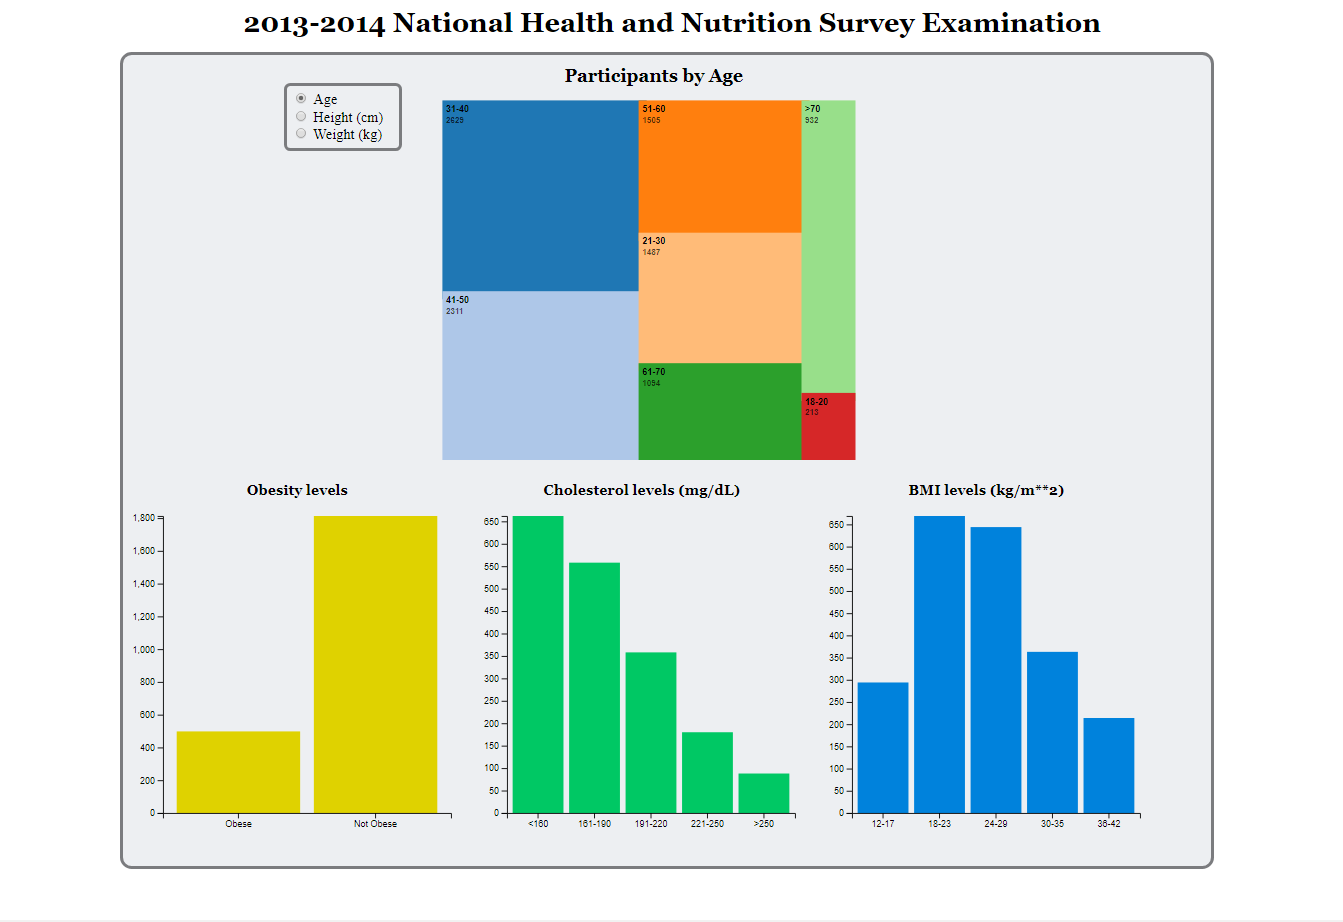
\includegraphics[scale=0.55]{CSC595P1.png}
\end{center}
\end{figure}

\newpage
 \begin{figure}[!hb]
\begin{center}
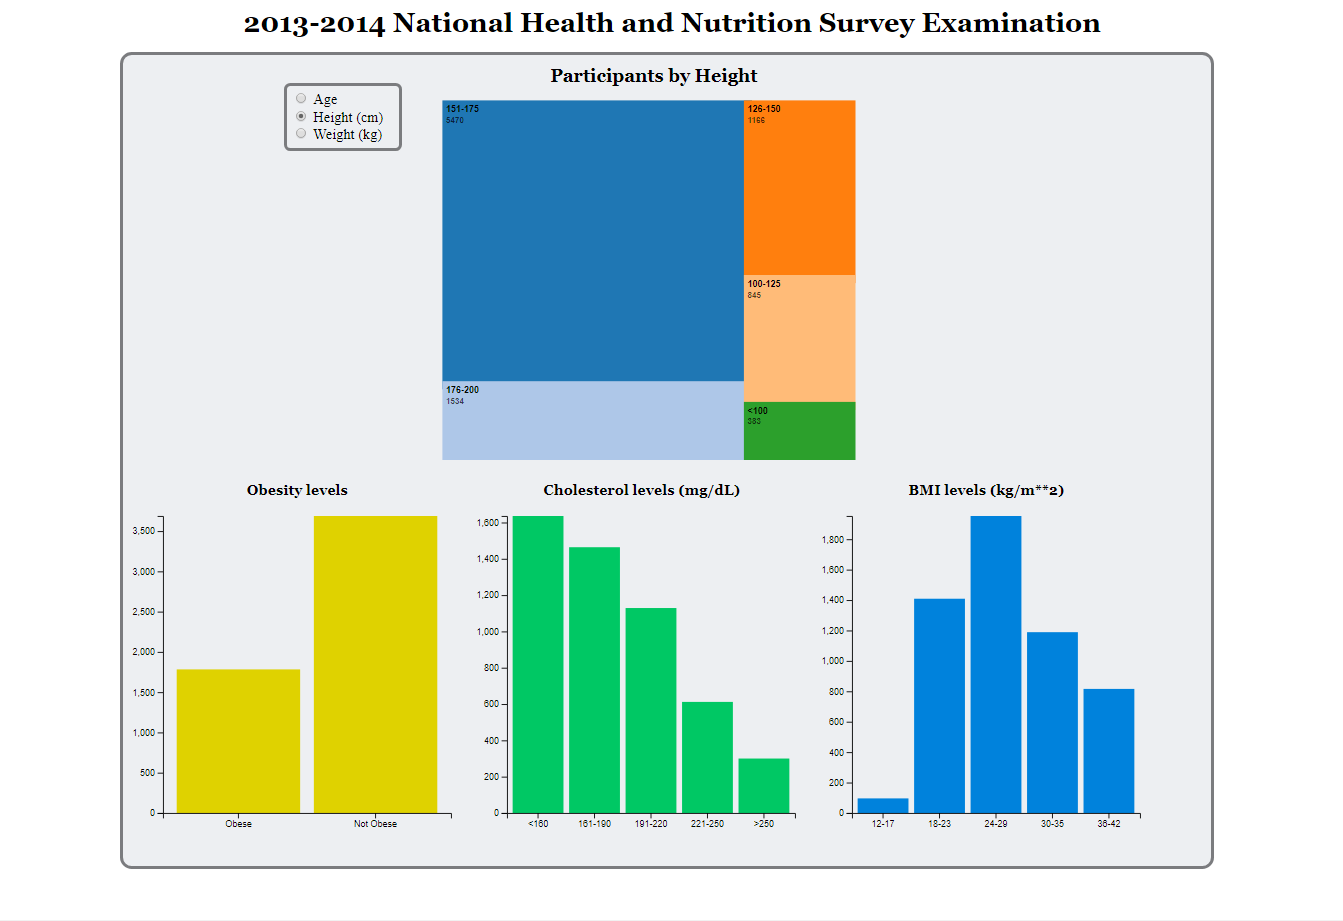
\includegraphics[scale=0.55]{CSC595P2.png}
\end{center}
\end{figure}
 \newpage



\newpage

{\section{Individual Reports}}
{\sf Kendall Zettlmeier}\\
The work that I did for the project, started with setting up the team with a GitHub repository where the team could collaborate on the project together and store all of our code and deliverables.  I also got the team started with deliverable 0 by creating the text file to be turned in and giving a description of the dataset that the team chose with a brief introduction on what we were going to be doing with the data.  I was also able to pull down some data via the Kaggle site to match multiple CSVs into 1 CSV by create an combined excel workbook and matching the survey participants SEQN numbers to each CSV via a VLOOKUP excel function.  As far as the actual implementation of the visualization goes, I was able to get the data setup in such a way to use age, weight, and height as heirarchical datasets in which we could create a treemap of the different data chunks.  By splitting the data for age, weight, and height into different groups, it made for visualizing the data into a more managable chunks.  I then set the 3 data chunks to be displayed via treemaps via a generic treemap helper that I created, and set the different treemaps to be viewed based upon the radio selection that was chosen.  I was also able to get the treemap dispatch function setup to send across the clicked group so that we could hook the click up to open up sub pie charts below the treemap.  After the presentation feedback, I changed the pie charts into bar charts, and I was able to make the conversion in code very easliy thanks to the way Kevin architected the pie charts javascript files.

As far as what I learned from the visualization, is was basically what I expected.  The younger the age group the lower the BMI and cholesterol levels were.  The younger the age, also had fewer obese survey participants.  Since there is a direct correlation to the height and weight to what the BMI was, it wasn't surprising to see that heavier weighted participants had a larger percentage of obesity and high cholesterol.  It was on the otherhand interesting to see the differences in height in which groups had higher amounts of obesity.  I did not necessarily think that the taller groups would have higher percentages of obesity.  I tend to think of most tall people as thin, so it was interesting to see that the tallst group had the highest obesity percentage.

{\sf Zachary Zimmer}\\
For the project my main component was writing the report. I structured the report around both the guidelines as well as my own knowledge. I also did a literature search to find interesting and relevant articles whichwould explain the background material or provide some understanding of the overarching NHANES dataset.This would meet the basics understanding of the data and the literature search provided the background material. For the other sections I focused on the suggestions from the assignment with emphases of the data, datacleaning (there was not much) and the actual visualization tool. The data was described in a table to explainthe key variables from the original source (I left off any variables derived outside the database). This showedthe variables name, type, units if continuous, levels if categorical, and a description. For the visualizationdescription I first described what the tool was, the thought process the team used for the layout, and then didsome summaries of the results. For the thought process and layout this described in detail how any why wechose the layout that we did to make the tool easy to use for a perspective user. This explained the layoutof the figures, the choice and color palette of the selection box, and any text included. For the summary Idescribed the relationship between the age bins and the variables obesity, BMI, and cholesterol. This wasthe most interesting comparison as there was an observable relationship between the age and these variable,acknowledging that this is based on observation as opposed to experimental data. Even with larger samplesizes one must be careful when making claims given how the data was collected.From this I learned more about D3 including the use if jQuery. This was incorporated in the use of theradial buttons for selecting the variables used in the main treemap. We had not used jQuery in the course. Italso emphasizes the use of bar charts versus pie charts for clarity. This emphasizes how in our case the use oflength was better than using pie charts even with some color to split the groups as good/low or bad/high forvariables like obesity or cholesterol.

{\sf Kevin Looft}\\
On the administrative side of the project, at the beginning I helped contribute with the rest of the team on research into which dataset we wanted to proceed with. Once it was decided, I organized a meeting with the team to discuss and create Deliverable 2, which was where we decided what types of visualizations we wanted to create and how they would interact with each other. The mockup I created here was used as the template for the start of our implementation. On the coding side, my work began on the sub charts of the visualization. I created the pie charts in our original visualization. Each of these charts (obesity, cholesterol levels, and BMI levels) were rendered after a dispatch event from a click on the main treemap which identified the selected dataset for the sub charts to include. In my code I had to check each of the rows in our original dataset to see if they were to be included in the sub chart, and then break them out into groups depending on which column was being used for that chart. The structure of the pie charts I created was easily changed into bar charts by Kendall following feedback we received in class. I also contributed to the overall styling of the application.

Regarding the data we chose, I don’t think there were many surprises based on the patterns we saw. The health indicators (obesity, cholesterol, BMI) generally trended towards more unhealthy with age and weight. The main learning I took away was more about how to display the data in order to show the correct message. We went through a few iterations just on paper about how to display our main group of data. We knew we wanted to have a split between age, height, and weight, and we debated a few different ways on how to show that. We agreed that a treemap would be a good fit, even though our data was not in the traditional hierarchical format typically found on a treemap it still worked for us. We also went through the same process with the sub charts. We started out with pie charts, but in agreement with the feedback we received we felt that bar charts would be better to show the difference between the different levels of cholesterol and BMI as well as obesity. This experience helped me learn that while a set of data might ‘fit’ into a particular chart, it might not be conveying a useful message inside that chart.

{\sf Harika Rallapalli}\\

{\sf Mohammadsaleh Gharehdaghi}\\

\newpage

{\sf References}

[1] Centers of Disease Control and Prevention. National diabetes factor sheet: national estimates and general information on diabetes and prediabetes in the United States, 2011. US Department of Health and Human Services, Centers for Disease Control and Prevention, 1(1), 2568-69.

[2] Choi, Jung U (2014). Obesity and its metabolic complications: the role of adipokines, inflammation, insulin resistance, dyslipidemia, and nonalcoholic fatty liver disease.  International Journal of Molecular Sciences, 15(4), 6184-6223.

[3] Ford ES (2005). Risks for all-cause mortality, cardiovascular disease, and diabetes associated with metabolic syndrome: a summary of the evidence, Diabetes Cares, 28(7), 1769-1778.

[4] Hales, CM, Carrol, MD, Fryar, CD, and Ogden, CL (2017). Prevalence of obesity among adults and youth: United States, 2015-2016.

[5] Howell, CR, Fontaine, K, Ejima, K, Ness, KK, et al (2017). Maximum lifetime body mass index and mortality in Mexican American adults: the National Health and Nutritional Examination Survey III (1988-1994) and NHANES 1999-2010. Preventing Chronic Disease, 1545-1151(14).

[6] Iranpour, S. and Sabour S (2019). Inverse Association between caffeine intake and depression symptoms in US adults: data from National Health and Nutritional Examination Survey (NHANES) 2005-2006. Psychiatry Research, 1872-7123(271), 732-739.

[7] Thompson, DR, Obarzanek, E, Franko, DL, Barton, BA, Morrison, J, Biro, FM, Daniels, SR, Striegel-Moore, RH (2007).  Childhood overweight and cardiovascular disease risk factors: the National Heart, Lung, and Blood Institute Growth and Health Study. The Journal of Pediatrics, 150(1), 18-25.

[8] Wang Q, Wei S (2018). Cadmium affects blood pressure and negatively interacts with obesity: Findings in the NHANES 1999-2014. The Science of the Total Environment, 1879-1026(643), 270-276.

[9] \url{https://www.cdc.gov/healthyweight/assessing/bmi/adult_bmi/index.html}



\end{document}
